\documentclass[conference]{IEEEtran}

\usepackage[utf8]{inputenc}
\usepackage[pdftex]{graphicx}
\usepackage{epstopdf}
\usepackage[hidelinks]{hyperref}
\usepackage{amssymb}
\usepackage{algorithm}
\usepackage{algorithmic}

\usepackage{flushend}

%%%%%%%%%%%%%%%%%%%%%%%%%%%%%%%%%%%%%%%%%%%%%%%%%%%%%%%%%%%%%%%%%%%%%%%%%%
% Definitions for comments
%%%%%%%%%%%%%%%%%%%%%%%%%%%%%%%%%%%%%%%%%%%%%%%%%%%%%%%%%%%%%%%%%%%%%%%%%%
% Marginpar redefinition
\let\oldmarginpar\marginpar
\renewcommand\marginpar[1]{\-\oldmarginpar[\raggedleft\footnotesize #1]%
{\raggedright\footnotesize #1}}
%%%%%%%%%%%%%%%%%%%%%%%%%%%%%%%%%%%%%%%%%%%%%%%%%%%%%%%%%%%%%%%%%%%%%%%%%%
\usepackage{mparhack}
\setlength{\marginparsep}{0.2cm}
\setlength{\marginparwidth}{1.8 cm}
\newenvironment{comment}[2][Note]{\dag\marginpar{\tiny{\textbf{#1:} {#2}}}}
%\newenvironment{comment}[2][Note]{}
%\newenvironment{comment}[2][Note]{\footnote{\textbf{#1:} #2}}
%%%%%%%%%%%%%%%%%%%%%%%%%%%%%%%%%%%%%%%%%%%%%%%%%%%%%%%%%%%%%%%%%%%%%%%%%%

%%%%%%%%%%%%%%%%%%%%%%%%%%%%%%%%%%%%%%%%%%%%%%%%%%%%%%%%%%%%%%%%%%%%%%%%%%
% Meta commenting macros from Felipe
%%%%%%%%%%%%%%%%%%%%%%%%%%%%%%%%%%%%%%%%%%%%%%%%%%%%%%%%%%%%%%%%%%%%%%%%%%
\usepackage[usenames]{xcolor}
\usepackage{hyperref}

\ifx\final\undefined
	% 
	\ifx\todo\undefined
	\newcommand\todo[1]{~\newline{\color{red}\framebox[\columnwidth]{\parbox{.95\columnwidth}{TODO: #1}}}~\newline}
	\fi
	% 
	\newcommand{\rev}[1]{\noindent\fbox{\parbox{.98\columnwidth}{\underline{NEEDS REFINING:}\\#1}}\\}
	\newcommand{\ask}[2]{\noindent{\bf (@#1:}~#2{\bf)}}
	\newcommand{\say}[2]{\noindent\fbox{\parbox{.98\columnwidth}{\noindent{\sc #1:}\\#2}}\\}
\else
	\newcommand{\rev}[1]{}
	\newcommand{\ask}[2]{}
	\newcommand{\say}[2]{}
	\newcommand\todo[1]{}
\fi
%%%%%%%%%%%%%%%%%%%%%%%%%%%%%%%%%%%%%%%%%%%%%%%%%%%%%%%%%%%%%%%%%%%%%%%%%%


\begin{document}

\title{Adaptive High-Level Strategy Learning in StarCraft}

\author{\IEEEauthorblockN{Jiéverson Maissiat}
 \IEEEauthorblockA{
 Faculdade de Informática\\
 Pontifícia Universidade Católica\\
 do Rio Grande do Sul (PUCRS)\\
 Email: contact@jieverson.com}
 \and
 \IEEEauthorblockN{Felipe Meneguzzi}
 \IEEEauthorblockA{
 Faculdade de Informática\\
 Pontifícia Universidade Católica\\
 do Rio Grande do Sul (PUCRS)\\
 Email: felipe.meneguzzi@pucrs.br}
}

%\author{
%	Paper \# 118825
%	\vspace*{6em}
%}

\maketitle

\begin{abstract}

Reinforcement learning (RL) is a technique to compute an optimal policy in stochastic settings whereby, actions from an initial policy are simulated (or directly executed) and the value of a state is updated based on the immediate rewards obtained as the policy is executed. 
Existing efforts model opponents in competitive games as elements of a stochastic environment and use RL to learn policies against such opponents. 
In this setting, the rate of change for state values monotonically decreases over time, as learning converges. 
Although this modeling assumes that the opponent strategy is static over time, such an assumption is too strong when human opponents are possible. 
Consequently, in this paper, we develop a meta-level RL mechanism that detects when an opponent changes strategy and allows the state-values to ``deconverge'' in order to learn how to play against a different strategy. 
We validate this approach empirically for high-level strategy selection in the \textit{Starcraft: Brood War} game.

\end{abstract}

%\IEEEpeerreviewmaketitle

%!TEX root = sbgames-metalearning.tex
\section{Introduction}
\label{sec:introduction}

Reinforcement learning is a technique often used to generate an optimal (or near-optimal) agent in a stochastic environment in the absence of knowledge about the reward function of this environment and the transition function~\cite{kaelbling1996reinforcement}. 
A number of algorithms and strategies for reinforcement learning have been proposed in the literature~\cite{stone2005reinforcement,graepel2004learningfight}, which have shown to be effective at learning policies in such environments. 
Some of these algorithms have been applied to the problem of playing computer games from the point of view of a regular player with promising results~\cite{taylor2011teachingmario,mohan2010ralationalmario}. 
However, traditional reinforcement learning often assumes that the environment remains static throughout the learning process so that when the learning algorithm converges. 
Under the assumption that the environment remains static over time, when the algorithm converges, the optimal policy has been computed, and no more learning is necessary. 
Therefore, a key element of RL algorithms in static environments is a learning-rate parameter that is expected to decrease monotonically until the learning converges. 
However, this assumption is clearly too strong when part of the environment being modeled includes an opponent player that can adapt its strategy over time. 
In this paper, we apply the concept of meta-level reasoning~\cite{cox2007metareasoning,ulam2008combining} to reinforcement learning~\cite{schweighofer2003meta} and allow an agent to react to changes of strategy by the opponent.
Our technique relies on using another reinforcement learning component to vary the learning rate as negative rewards are obtained after the policy converges, allowing our player agent to deal with changes in the environment induced by changing strategies of competing players.

This paper is organized as follows: in Section~\ref{sec:background} we review the main concepts used in required for this paper:
the different kinds of environments (\ref{subsec:environments}), 
some concepts of machine learning (\ref{subsec:machine-learning}) and
reinforcement learning (\ref{subsec:rl}); in Section~\ref{sec:sc} we explain the StarCraft game domain, 
and in Section~\ref{sec:meta-rl} we describe our solution.
Finally, we demonstrate the effectiveness of our algorithms through empirical experiments and results in Section~\ref{sec:results}.

%!TEX root = sbgames-metalearning.tex
\section{Background}
\label{sec:background}



\subsection{Environments}
\label{subsec:environments}

In the context of multi-agent systems, the environment is the world in which agents act.
The design of an agent-based system must take into consideration the environment in which the agents are expected to act, since it determines which AI techniques are needed for the resulting agents to accomplish their design goals. 
Environments are often classified according to the following attributes~\cite{russell1995artificial}:  observability, determinism, dynamicity, discreteness, and the number of agents. 

The first way to classify an environment is related to its observability. 
An environment can be unobservable, partially observable, or fully observable. 
For example, the real world is partially observable, since each person can only perceive what is around his or herself, and usually only artificial environments are fully observable.
% 
The second way to classify an environment, is about its determinism.
In general, an environment can be classified as stochastic or deterministic.
In deterministic environments, an agent that performs an action $a$ in a state $s$ always result in a transition to the same state $s'$, no matter how many times the process is repeated, whereas in stochastic environments there can be multiple possible resulting states $s'$, each of which has a specific transition probability.
% 
The third way to classify an environment is about its dynamics. 
Static environments do not change their transition dynamics over time, while dynamic environments may change their transition function over time. 
% 
Moreover an environment can be classified as continuous or discrete.
Discrete environments have a countable number of possible states, while continuous environments have an infinite number of states.
A good example of discrete environment is a chessboard, while a good example of continuous environment is a real-world football pitch. 
% 
Finally, environments are classified by the number of agents acting concurrently, as either single-agent or multi-agent. 
In single-agent environments, the agent operates by itself in the system (no other agent modifies the environment concurrently) while in multi-agent environments agents can act simultaneously, competing or cooperating with each other. 
A crossword game is a single-agent environment whereas a chess game is a multi-agent environment, where  two agents take turns acting in a competitive setting.



\subsection{Machine Learning}
\label{subsec:machine-learning}

An agent is said to be learning if it improves its performance after observing the world around it~\cite{russell1995artificial}. 
Common issues in the use of learning in computer games include questions such as whether to use learning at all, or wether or not insert improvement directly into the agent code if it is possible to improve the performance of an agent. 
Russell and Norvig~\cite{russell1995artificial} state that it is not always possible or desirable, to directly code improvements into an agent's behavior for a number of reasons. First, in most environments, it is difficult to enumerate all situations an agent may find itself in. Furthermore, in dynamic environments, it is often impossible to predict all the changes over time. And finally, the programmer often has no idea of an algorithmic solution to the problem. 

Thus, in order to create computer programs that change behavior with experience, learning algorithms are employed. 
There are three main methods of learning, depending on the feedback available to the agent. 
In \emph{supervised learning}, the agent approximates a function of input/output from observed examples. 
In \emph{unsupervised learning}, the agent learns patterns of information without knowledge of the expected classification. 
In \emph{reinforcement learning}, the agent learns optimal behavior by acting on the environment and observing/experiencing rewards and punishments for its actions. 
In this paper, we focus in reinforcement learning technique. 



\subsection{Reinforcement Learning}
\label{subsec:rl}

When an agent carries out an unknown task for the first time, it does not know exactly whether it is making good or bad decisions. 
Over time, the agent makes a mixture of optimal, near optimal, or completely suboptimal decisions. 
By making these decisions and analyzing the results of each action, it can learn the best actions at each state in the environment, and eventually discover what the best action for each state is. 

Reinforcement learning (RL) is a learning technique for agents acting in a stochastic, dynamic and partially observable environments, observing the reached states and the received rewards at each step~\cite{sutton1998reinforcement}. 
Figure~\ref{fig:rl} illustrates the basic process of reinforcement learning, where the agent performs actions, and learns from their feedback. 
An RL agent is assumed to select actions following a mapping of each possible environment state to an action. 
This mapping of states to actions is called a \emph{policy}, and reinforcement learning algorithms aim to find the \emph{optimal policy} for an agent, that is, a policy that ensure long term optimal rewards for each state. 

\begin{figure}[ht]
\centering
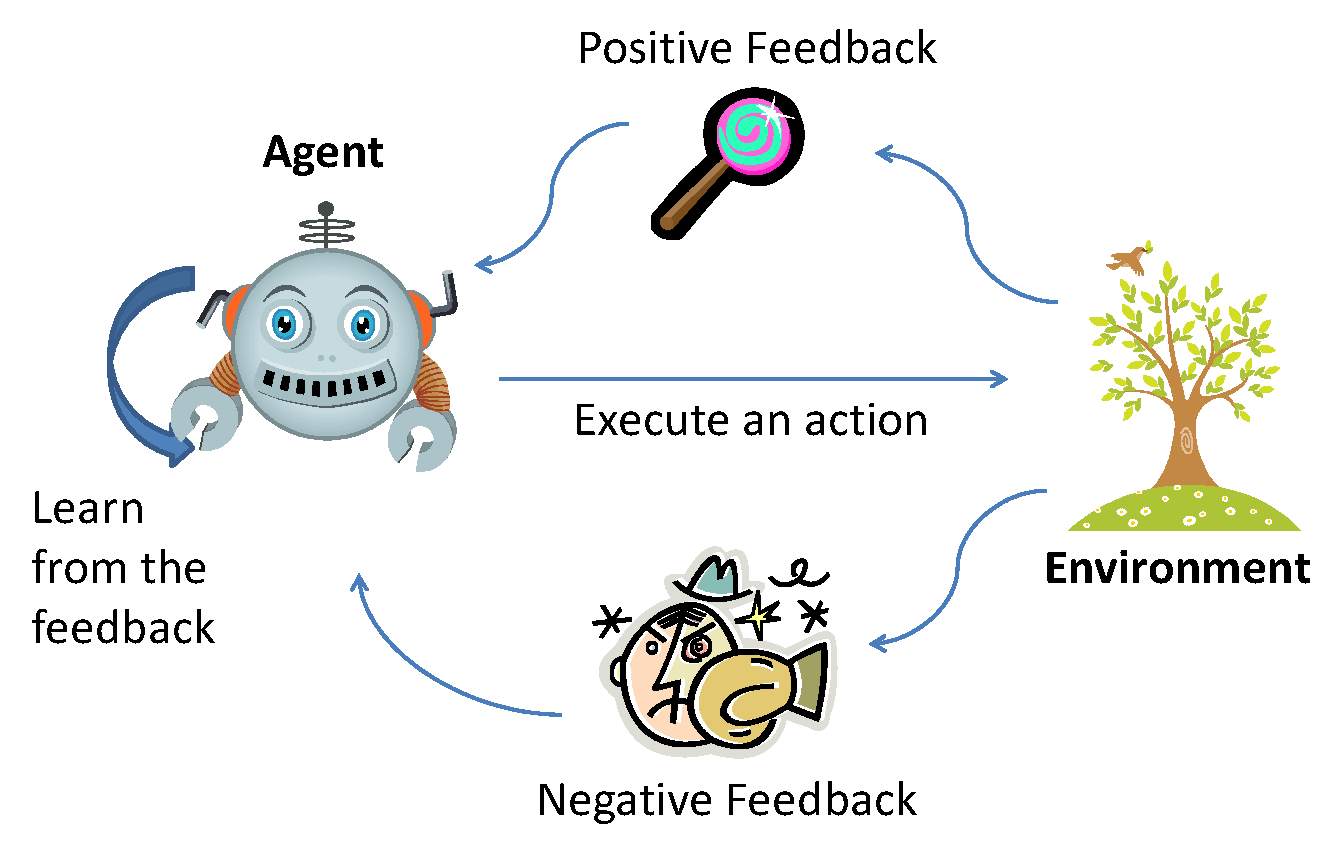
\includegraphics[width=250px]{images/rl}
\caption{Model to describe the process of reinforcement learning.}
\label{fig:rl}
\end{figure}

RL techniques are divided into two types, depending on whether the agent changes acts on the knowledge gained during policy execution~\cite{russell1995artificial}. 
In \emph{passive RL}, the agent simply executes a policy using the rewards obtained to update the \emph{value} (long term reward) of each state, whereas in \emph{active RL}, the agent uses the new values to change its policy on every iteration of the learning algorithm. 
A passive agent has fixed policy: at state $s$, the agent always performs the same action $a$.
Its mission is to learn how good its policy is $-$ to learn the utility of it.
An active agent has to decide what actions to take in each state:
it uses the information obtained by reinforcement learning to improve its policy. 
By changing its policy in response to learned values, an RL agent might start exploring different parts of the environment. 
Nevertheless, the initial policy still biases the agent to visit certain parts of the environment~\cite{russell1995artificial}, so an agent needs to have a policy to balance the use of recently acquired knowledge about visited states with the exploration of unknown states in order to approximate the optimal values~\cite{ghory2004boardgames}. 



\subsubsection{Q-Learning}
\label{subsubsec:ql}

Depending on the assumptions about the agent knowledge prior to learning, different algorithms are used. 
When the rewards and the transitions are unknown, one of the most popular reinforcement learning techniques is \textit{Q-learning}. 
This method updates the value of a pair of state and action --- named state-action pair, $Q(s,a)$ ---
after each action performed using the immediately reward. 
When an action $a$ is taken at a state $s$, the value of state-action pair, or Q-value,
is updated using the following adjustment function~\cite{amato2010highlevel}.
% 
	$$Q(s,a) \leftarrow Q(s,a) + \alpha[r + \gamma max_{a' \in A(s')}Q(s',a') - Q(s,a)]$$
% 

Where, 
\begin{itemize}
\item $s$ represents the current state of the world;
\item $a$ represents the action chosen by the agent;
\item $ Q(s,a) $ represents the value obtained the last time action $a$ was executed at state $s$.
This value is often called Q-value.
\item $r$ represents the reward obtained after performing action $a$ in state $s$;
\item $s'$ represents the state reached after performing action $a$ in state $s$;
\item $a' \in A(s')$ represents a possible action from state $s'$;
\item $max_{a' \in A(s')}Q(s',a')$ represents the maximum Q-value that can be obtained from the state $s'$, independently of the action chosen;
\item $\alpha$ is the learning-rate, which determines the weight of new information over what the agent already knows --- a factor of $0$ prevents the agent from learning anything (by keeping the Q-value identical to its previous value) whereas a factor of $1$ makes the agent consider all newly obtained information;
\item $\gamma$ is the \textit{discount factor}, which determines the importance of future rewards --- a factor of $0$ makes the agent opportunistic~\cite{schweighofer2003meta} by considering only the current reward, while a factor of $1$ makes the agent consider future rewards, seeking to increase their long-term rewards;
\end{itemize}

Once the Q-values are computed, an agent can extract the best policy known so far ($\pi^{\approx}$) by selecting the actions that yield the highest expected rewards using the following rule:
$$\pi^{\approx}(s) = \arg\max_{a}Q(s,a) $$

In dynamic environments, Q-learning does not guarantee convergence to the optimal policy.
This occurs because the environment is always changing and demanding that the agent adapts to new transition and reward functions.
However, Q-learning has been proven efficient in stochastic environments 
even without convergence~\cite{sandholm1996multiagent,tesauro2002pricing,amato2010highlevel}.
In multi-agent systems where the learning agent models the behavior of all other agents as a stochastic environment (an MDP), Q-learning provides the optimal solution when these other agents
-- or players in the case of human agents in computer games --- do not change their policy choice. 



\subsubsection{Exploration Policy}
\label{subsubsec:exploration}

So far, we have considered active RL agents that simply use the knowledge obtained so far to compute an optimal policy. 
However, as we saw before, the initial policy biases the parts of the state-space through which an agent eventually explores, possibly leading the learning algorithm to converge on a policy that is optimal for the states visited so far, but not optimal overall (a local maximum). 
Therefore, active RL algorithms must include some mechanism to allow an agent to choose different actions from those computed with incomplete knowledge of the state-space. 
Such a mechanism must seek to balance exploration of unknown states and exploitation of the currently available knowledge, allowing the agent both to take advantage of actions he knows are optimal, and exploring new actions~\cite{amato2010highlevel}. 

In this paper we use an exploration mechanism known as $\epsilon$-greedy~\cite{rodrigues2009dynamic}. 
This mechanism has a probability $\epsilon$ to select a random action, and a probability $1 - \epsilon$ to select the optimal action known so far --- which has the highest Q-value.
In order to make this selection we define a probability vector over the action set of the agent for each state, and use this probability vector to bias the choice of actions towards unexplored states. 
In the probability vector $x = (x_1, x_2, ..., x_n)$, the probability $x_i$ to choose the action $i$ is given by: 
\[
  x_i = \left\{
  \begin{array}{ll}
    (1 - \epsilon) + (\epsilon / n), & \mbox{if $Q$ of $i$ is the highest} \\
    \epsilon / n, & \mbox{otherwise}
  \end{array}\right.
\]

where $n$ is the number of actions in the set.



\subsection{Meta-Level Reasoning}
\label{subsec:meta-reasoning}

Traditionally, \textit{reasoning} is modeled as a decision cycle, in which the agent perceives environmental stimulus and responds to it with an appropriate action. 
The result of the actions performed in the environment (\textit{ground-level})
is perceived by the agent (\textit{object-level}), which responds with a new action,
and so the cycle continues. 
This reasoning cycle is illustrated in Figure~\ref{fig:reasoning}~\cite{cox2007metareasoning}. 

\begin{figure}[ht]
\centering
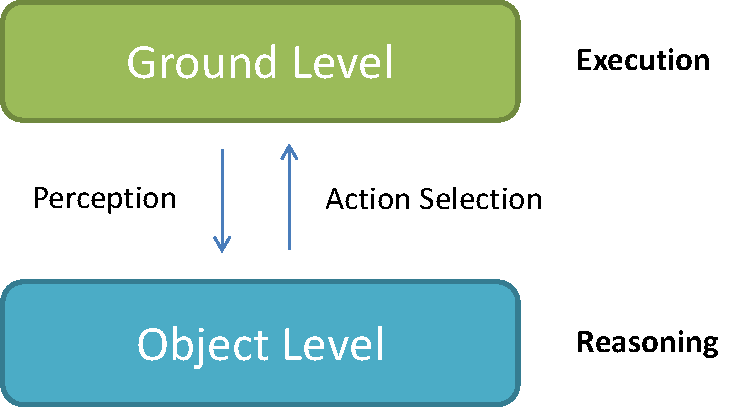
\includegraphics[width=230px]{images/reasoning}
\caption{Common cycle of perception and actions choice.}
\label{fig:reasoning}
\end{figure}

\textit{Meta-reasoning} or \textit{meta-level reasoning} is the process of explicitly reasoning about this reasoning cycle. 
It consists of both the control, and monitoring of the object-level reasoning, allowing an agent to adapt the reasoning cycle over time, as illustrated in Figure~\ref{fig:metareasoning}. 
This new cycle represents a high level reflection about its own reasoning cycle. 

\begin{figure}[ht]
\centering
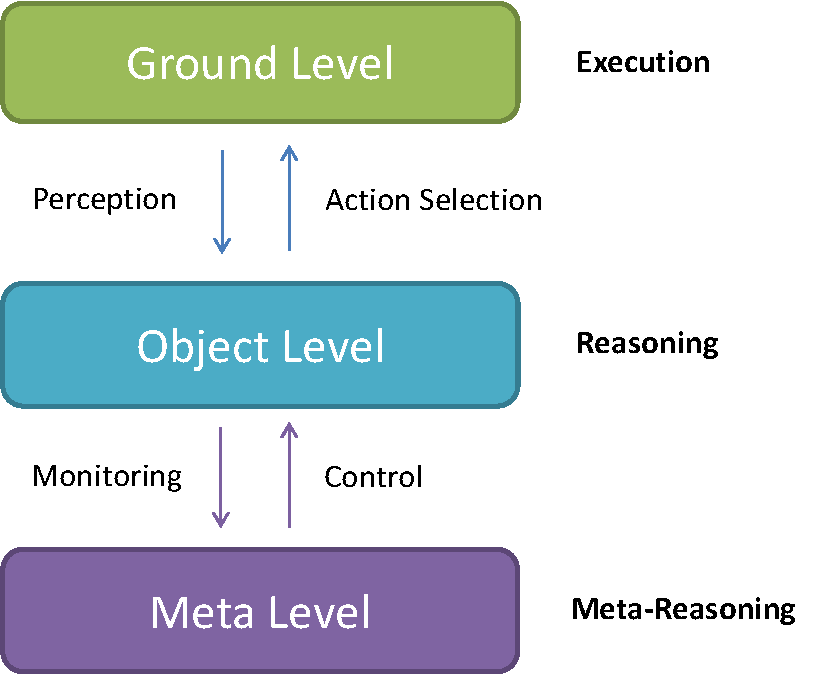
\includegraphics[width=230px]{images/metareasoning}
\caption{Adding meta-level reasoning to the common cycle of perception and choice of actions.}
\label{fig:metareasoning}
\end{figure}

When meta-level reasoning is applied to learning algorithms, this gives rise to a new term: \textit{meta-learning}~\cite{schweighofer2003meta, doya2002metalearning}.
Meta-learning represents the concept of learning to learn, and the meta-learning level is generally responsible for controlling the parameters of the learning level.
While learning at the object-level is responsible for accumulating experience about some task (e.g, take decisions in a game, medical diagnosis, fraud detection, etc.), learning at the meta-level is responsible for accumulating experience about learning algorithm itself. 
If learning at object-level is not succeeding in improving or maintaining performance, the meta-level learner takes the responsibility to adapt the object-level, in order to make it succeed.
In other words, meta-learning helps solve important problems in the application of machine learning algorithms~\cite{vilalta2004using}, especially in dynamic environments.

%!TEX root = sbgames-metalearning.tex
\section{StarCraft}
\label{sec:sc}

\emph{Real-time strategy} (RTS) games are computer games in which multiple players control teams of characters and resources over complex simulated worlds where their actions occur simultaneously (so there is no turn-taking between players). 
Players often compete over limited resources in order to strengthen their team and win the match. 
As such RTS games are an interesting field for the AI, because the state space is huge, actions are concurrent, and part of the game state is hidden from each player. 
Game-play involves both the ability to manage each unit individually \textit{micro-management}, and a high-level strategy for building construction and resource gathering (\textit{macro-management}). 

\textit{StarCraft} is an RTS created by \textit{Blizzard Entertainment, Inc.}\footnote{
StarCraft website in Blizzard Entertainment, Inc. \url{http://us.blizzard.com/pt-br/games/sc/}}.
In this game, a player chooses between three different races to play (illustrated in Figure~\ref{fig:sc-races}), each of which having different units, buildings and capabilities, and uses these resources to battle other players, as shown in Figure~\ref{fig:sc-fight}. 
% 
\begin{figure}[ht]
\centering
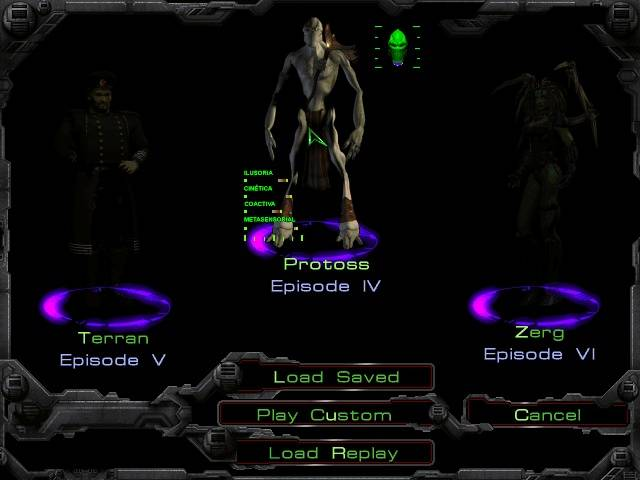
\includegraphics[width=250px]{images/sc-races}
\caption{StarCraft: Brood War $-$ Race selection screen.}
\label{fig:sc-races}
\end{figure}
% 
The game consists on managing resources and building an army of different units to compete against the armies built by opposing players. 
Units in the game are created from structures, and there are prerequisites for building other units and structures. 
Consequently, one key aspect of the game is the order in which buildings and units are built, and good players have strategies to build them so that specific units are available at specific times for attack and defense moves. 
These building strategies are called \textit{build orders} or \textit{BOs}. 
Strong BOs can put a player in a good position for the rest of the match.
BOs usually need to be improvised from the first contact with the enemy units, since the actions become more dependent on knowledge obtained about the units and buildings available to the opponent~\cite{hagelback2012potential,churchill2011build}. 
% 
\begin{figure}[ht]
\centering
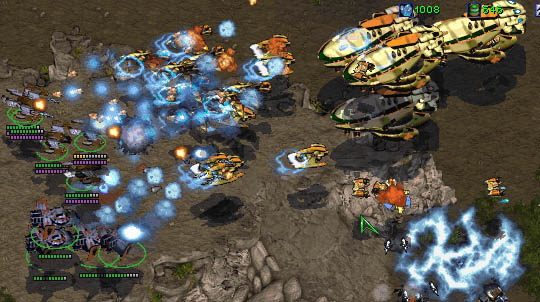
\includegraphics[width=250px]{images/sc-fight}
\caption{StarCraft: Brood War $-$ Batttle Scene.}
\label{fig:sc-fight}
\end{figure}

%!TEX root = sbgames-metalearning.tex
\section{Meta-Level Reinforcement Learning}
\label{sec:meta-rl}



\subsection{Parameter Control}
\label{subsec:parameter-control}

As we have seen in Section~\ref{subsec:rl}, the parameters used in the update rule of reinforcement learning influence how the state values are computed, and ultimately how a policy is generated. 
Therefore, the choice of the parameters in reinforcement learning
--- such as $\alpha$ and $\gamma$ ---
can be crucial to success in learning~\cite{schweighofer2003meta}. 
Consequently, there are different strategies to control and adjust these parameters. 

When an agent does not know much about the environment, it needs to explore the environment with a high learning-rate to be able to quickly learn the actual values of each state. 
However, a high learning-rate can either prevent the algorithm from converging, or lead to inaccuracies in the computed value of each state (e.g. a local maximum). 
For this reason, after the agent learns something about the environment, it should begin to modulate its learning-rate to ensure that either the state values converge, or that the agent overcomes local maxima. 
% 
Consequently, maintaining a high learning-rate hampers the convergence of the Q-value, and Q-learning implementations often use a decreasing function for $\alpha$ as the policy is being refined. 
A typical way~\cite{schweighofer2003meta} to vary the $\alpha$-value, is to start interactions with a value close to $1$, and then decrease it over time toward $0$.
However, this approach is not effective for dynamic environments, since a drastic change in the environment with a learning-rate close to $0$ prevents the agent from learning the optimal policy in the changed environment. 



\subsection{Meta-Level Reasoning on Reinforcement Learning}
\label{subsec:meta-reasoning-rl}

The objective of meta-level reasoning is to improve the quality of decision making by explicitly reasoning about the parameters of the decision-making process and deciding how to change these parameters in response to the agent's performance. 
Consequently, an agent needs to obtain information about its own reasoning process to reason effectively at the meta-level. 
In this paper, we consider the following processes used by our learning agent at each level of reasoning, and illustrate these levels in Figure~\ref{fig:reasoningOnRL}:

\begin{itemize}
\item \textit{ground-level} refers to the implementation of actions according to the MDP's policy;
\item \textit{object-level} refers to learning the parameters of the MDP and the policy itself;
\item \textit{meta-level} refers to manipulating the learning parameters used in \textit{object-level};
\end{itemize}

\begin{figure}[ht]
\centering
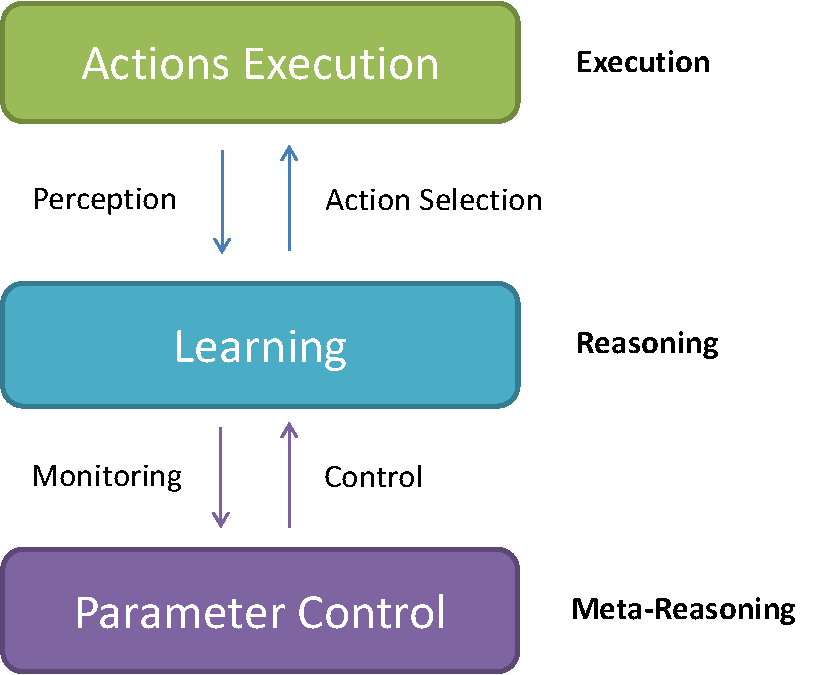
\includegraphics[width=230px]{images/reasoningOnRL}
\caption{Modeling the meta-level reasoning in reinforcement learning.}
\label{fig:reasoningOnRL}
\end{figure}

Our approach to meta-level reasoning consists of varying the learning-rate (known as $\alpha-$value)
to allow an agent to handle dynamic environments. 
More concretely, at the meta-level, we apply RL to learn the $\alpha-$value used as the learning-rate at the object-level RL. 
In other words, we apply reinforcement learning to control the parameters of reinforcement learning. 

The difference between RL applied at the meta-level and RL applied at the object-level is that, at the object-level, we learn Q-value for the action-state pair, increasing it when we have positive feedback and decreasing it when we have negative feedback. 
Conversely, at the meta-level, what we learn in the $\alpha$-value, by decreasing it when we have positive feedback and increasing it when we have negative feedback --- that is, making mistakes means we need to learn at a faster rate. 
Our approach to \textit{meta-level reinforcement learning} is shown in Algorithm~\ref{alg:meta-rl}. 

\begin{algorithm}
	\caption{Meta-Level Reinforcement Learning}
	\label{alg:meta-rl} 
	\begin{algorithmic}[1]
		\REQUIRE $s, a, R$
		\STATE $\alpha \gets \alpha - (0.05 * R)$ \label{meta-rl:line:meta-level}
		\item[]
		\IF{$\alpha < 0$} \label{meta-rl:line:alpha-begin}
			\STATE $\alpha \gets 0$
		\ENDIF
		\IF{$\alpha > 1$}
			\STATE $\alpha \gets 1$
		\ENDIF \label{meta-rl:line:alpha-end}
		\item[]
		\STATE $Q(s,a) \gets Q(s,a) + (\alpha * R)$ \label{meta-rl:line:qlearning}
	\end{algorithmic}
\end{algorithm}

The meta-level reinforcement learning algorithm requires the same parameters as Q-learning:
a state $s$, an action $a$ and a reward $R$.
In Line~\ref{meta-rl:line:meta-level} we apply the RL update rule for the $\alpha$-value used for the object-level Q-learning algorithm. 
At this point, we are learning the learning-rate, and as we saw, $\alpha$ decreases with positive rewards. 
We use a small constant learning-rate of $0.05$ for the meta-level update rule and bound it between $0$ and $1$ (Lines~\ref{meta-rl:line:alpha-begin}--\ref{meta-rl:line:alpha-end}) to ensure it remains a consistent learning-rate value for Q-learning. 
Such a small learning-rate at the meta-level aims to ensure that while we are constantly updating the object-level learning-rate, we avoid high variations. 
Finally, in Line~\ref{meta-rl:line:qlearning} we use the standard update rule for Q-learning,
using the adapted learning-rate. 
As the algorithm is nothing but a sequence of mathematical operations, it is really efficient when it comes to time. 
Thus, it is able to execute in few clock cycles and could be utilized in real-time after each action execution.

Since we are modifying the learning-rate based on the feedback obtained by the agent, and increasing it when the agent detects that its knowledge is no longer up to date, we can also use this value to guide the exploration policy. 
Thus, we also modify the $\epsilon-$greedy action selection algorithm.
Instead of keeping the exploitation-rate ($\epsilon-$value) constant, we apply the same meta-level reasoning to the $\epsilon-$value, increasing the exploration rate, whenever we find that the agent must increase its learning-rate ---  the more the agent wants to learn, the more it wants to explore;
if there is nothing to learn, there is nothing to explore.
To accomplish this, we define the exploitation-rate as been always equal to the learning-rate:
\[
	\epsilon = \alpha
\]





%!TEX root = sbgames-metalearning.tex
\section{Experiments and Results}
\label{sec:results}

In this section, we detail our implementation of meta-level reinforcement learning and its integration to the \emph{Starcraft} game, followed by our experiments and their results. 



\subsection{Interacting with StarCraft}
\label{subsec:bwapi}

The first challenge in implementing the algorithm is the integration of our learning algorithm to the proprietary code from Starcraft, since we cannot directly modify its code and need external tools to do this. 
In the case of StarCraft, community members developed the \textit{BWAPI}, which allows us to inject code into the existing game binaries. 
The \textit{BWAPI (Brood War Application Programming Interface)}\footnote{An API to interact with StarCraft: BroodWar \url{http://code.google.com/p/bwapi/}} enables the creation and injection of artificial intelligence code into StarCraft. 
BWAPI was initially developed in \textit{C++}, and later ported to other languages like \textit{Java}, \textit{C\#} and \textit{Python}, and divides StarCraft in 4 basic types of object:


\begin{itemize}
\item \textit{Game:} manages information about the current game being played, 
including the position of known units, location of resources, etc.;
\item \textit{Player:} manages the information available to a player, such as: 
available resources, buildings and controllable units;
\item \textit{Unit:} represents a piece in the game, either mineral, construction or combat unit;
\item \textit{Bullet:} represents a projectile fired from a ranged unit;
\end{itemize}

Since the emergence of BWAPI in 2009, StarCraft has drawn the attention of researchers and an active community of bot programming has emerged~\cite{buro2012real}. 
For our implementation, we modified the open source bot \textit{BTHAI}~\cite{hagelback2012potential},
adding a high-level strategy learning component to it\footnote{The source code can be fount at: \url{https://github.com/jieverson/BTHAIMOD}}.
Figure~\ref{fig:game-play} shows a screenshot of a game where one of the players is controlled by BTHAI, notice the additional information overlaid on the game interface. 

\begin{figure}[ht]
\centering
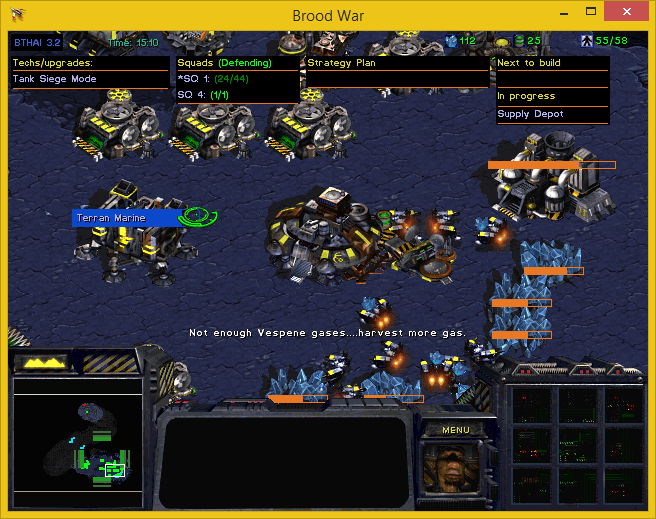
\includegraphics[width=250px]{images/game-play}
\caption{BTHAI bot playing StarCraft: Brood War.}
\label{fig:game-play}
\end{figure}



\subsection{A Reinforcement Learning Approach for StarCraft}
\label{subsec:rl-sc}

Following the approach used by~\cite{amato2010highlevel}, our approach focuses on learning the best high-level strategy to use against an opponent. 
We assume here that the agent will only play as Terran, and will be able to choose any one of the following strategies:

\begin{itemize}
\item \textit{Marine Rush:} is a very simple Terran strategy that relies on quickly creating a specific number of workers (just enough to maintain the army) and then spending all the acquired resources on the creation of Marines (the cheapest Terran battle unit) and making an early attack with a large amount of units.

\item \textit{Wraith Harass:} is similar, but slightly improved, Marine rush that consists of adding 
a mixture of 2--5 Wraiths (a relatively expensive flying unit) to the group of Marines. The Wraith's mission is to attack the opponent from a safe distance, and when any of the Wraiths are in danger,  use some Marines to protect it.
Unlike the Marine Rush, this strategy requires strong micromanagement, making it more difficult to perform. 

\item \textit{Terran Defensive:} consists of playing defensively and waiting for the opponent to attack before counterattacking. 
Combat units used in this strategy are Marines and Medics (a support unit that can heal biological units),
usually defended by a rearguard of Siege Tanks.

\item \textit{Terran Defensive FB:} is slightly modified version of the Terran Defensive strategy, which replaces up to half of the Marines by Firebats --- a unit equipped with flamethrowers that is 
especially strong against non-organic units such as aircrafts, tanks and most of Protoss' units.

\item \textit{Terran Push:} consists of creating approximately five Siege Tanks and a large group of Marines, and moving these units together through the map in stages, stopping at regular intervals to regroup. 
Given the long range of the Tank's weapons, opponents will often not perceive their approach until their units are under fire, however, this setup is vulnerable to air counterattack units. 
\end{itemize}

After each game, the agent observes the end result (victory or defeat), and uses this feedback to learn the best strategy. 
If the game is played again, the learning continues, so we can choose the strategy with the highest value for the current situation. 
If the agent perceives, at any time, that the strategy ceases to be effective 
--- because of a change in the opponent's strategy, map type, race or other factors ---
the agent is able to quickly readapt to the new conditions, choosing a new strategy.



\subsection{Experiments with StarCraft}
\label{subsec:experiments}

To demonstrate the applicability of our approach we have designed an experiment whereby a number of games are played against a single opponent that can play using different AI bot strategies. 
We seek to determine if our learning methods can adapt its policy when the AI bot changes. 
Each game was played in a small two-player map (\textit{Fading Realm}) using the maximum game speed (since all players were automated).
The game was configured to start another match as soon as the current one ends.
For the experiment, all the Q-values are initialized to $0$, and the learning-rate ($\alpha$) is initialized to $0.5$. 
Our experiment consisted of playing the game a total of 138 matches where one of the players is controlled by an implementation of our meta-learning agent. 
In the first $55$ matches, the opponent have played a fixed Terrain policy provided by the game and in subsequent matches, we have changed the opponent policy to the fixed Protoss policy provided by the game. 
It is worth noting that our method used very little computation time--it runs in real time, using accelerated game speed (for matches between two bots).

\begin{figure}[ht]
\centering
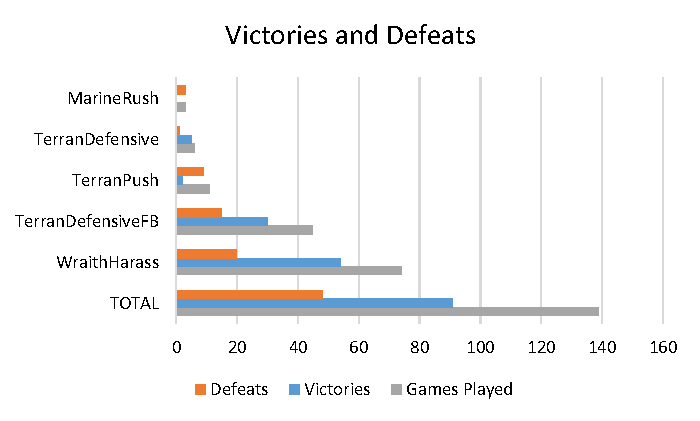
\includegraphics[width=250px]{images/wins_graphic}
\caption{Comparison between the number of victories and defeats of each strategy.}
\label{fig:wins_graphic}
\end{figure}

\begin{figure}[ht]
\centering
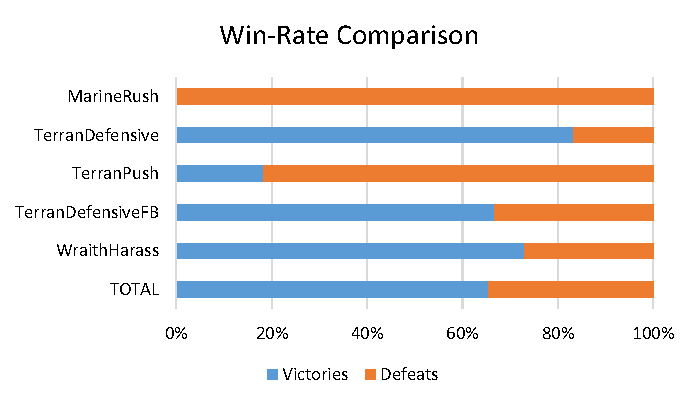
\includegraphics[width=250px]{images/win-rates_graphic}
\caption{Graphic that presents a comparation between the win rate of each strategy.}
\label{fig:win-rates_graphic}
\end{figure}

The results obtained are illustrated in the graph of Figure~\ref{fig:wins_graphic} and Figure~\ref{fig:win-rates_graphic}, which shows that our meta-learning agent consistently outperforms fixed opponents. 
Moreover, we can see that the agent quickly learns the best strategy to win against a fixed policy opponent when its strategy changes. 
As it learns, its learning-rate should tend to decrease towards $0$, which means that the agent has nothing to learn.
After the change in opponent policy (at game execution $55$), we expected the learning-rate to   increase, denoting that the agent is starting to learn again, which was indeed the case, as illustrated by the graph of Figure~\ref{fig:learning-rate_graphic}. 
The learning rate should remain above $0$ until the RL algorithm converges to the optimal policy, and then start decreasing towards $0$.
We note that, although the learning-rate may vary between $0$ and $1$, it has never gone beyond $0.7$ in the executions we performed.

\begin{figure}[ht]
\centering
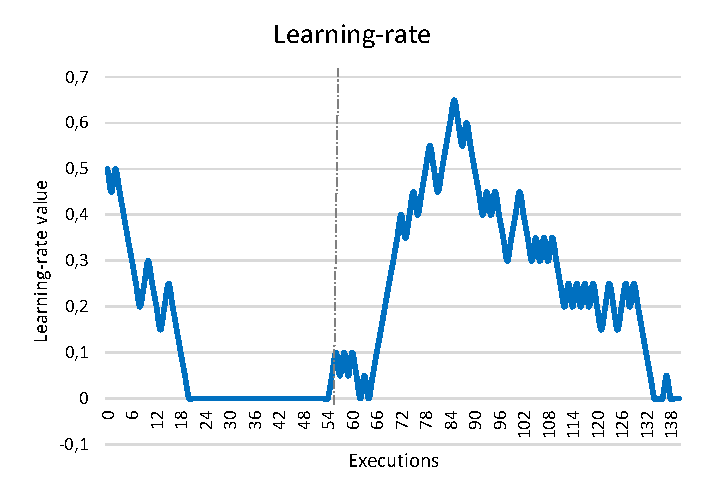
\includegraphics[width=250px]{images/learning-rate_graphic}
\caption{Learning-rate variation over time.}
\label{fig:learning-rate_graphic}
\end{figure}

Finally, the graphic in Figure~\ref{fig:strategies_graphic} illustrates the variation
of the strategies Q-values over each game execution.
We can see that the \textit{Wraith Harass} strategy was optimal against the first opponent policy, 
while the \textit{Terrain Push} has proven to be the worst.
When the opponent changes its policy, we can see the Q-value of \textit{Wraith Harass} decreases,
resulting in an increase in exploration. 
After the execution $85$, we notice that the \textit{Terrain Defensive FB} strategy stood out from the others, although the basic \textit{Terrain Defensive} strategy has shown to yield good results too. 
\textit{Wraith Harass} and \textit{Marine Rush} seem to lose to the second opponent policy, 
and \textit{Terrain Push} shows remain the worst strategy. 

\begin{figure}[ht]
\centering
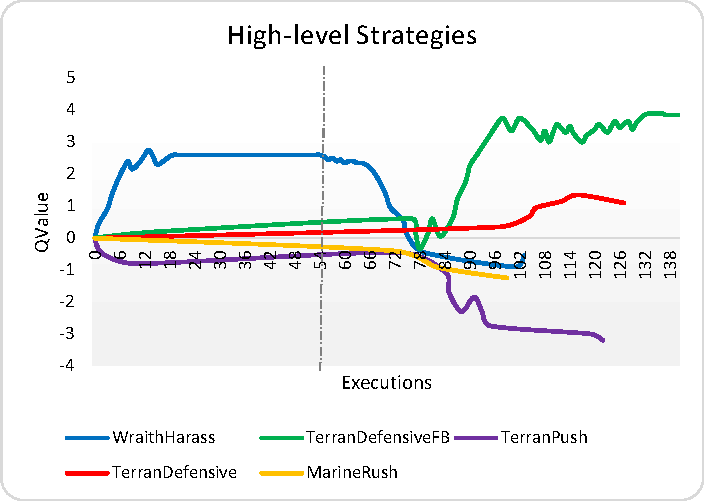
\includegraphics[width=250px]{images/strategies_graphic}
\caption{Strategies Q-Value over time.}
\label{fig:strategies_graphic}
\end{figure}

%!TEX root = sbgames-metalearning.tex
\section{Conclusion}
\label{sec:conclusion}

In this paper we have developed a reinforcement learning mechanism for high-level strategies in RTS games that is able to cope with the opponent abruptly changing its play style. 
To accomplish this, we have applied meta-level reasoning techniques over the already known RL strategies, so that we learn how to vary the parameters of reinforcement learning allowing the algorithm to ``de-converge'' when necessary.
The aim of our technique is to learn when the agent needs to learn faster or slower. 
Although we have obtained promising initial results, our approach was applied just for high-level strategies, and the results were collected using only the strategies built into the BTHAI library for Starcraft control.
To our knowledge, ours is the first approach to mix meta-level reasoning and reinforcement learning that applies RL to control the parameters of RL.
The results have shown that this meta-level strategy can be a good solution to find high-level strategies.
The meta-learning algorithm we developed is not restricted to StarCraft and can be used in any game in which the choice of different strategies may result in different outcomes (victory or defeat), based on the play style of the opponent. 
In the future, we aim to apply this approach to low-level strategies, such as learning detailed \textit{build orders} or to micro-manage battles.
Given our initial results, we believe that meta-level reinforcement learning is a useful technique in game AI control that can be used on other games, at least at a strategic level. 

\section*{Acknowledgment}
\label{sec:acknowledgment}

The authors would like to thank the members of the BTHAI and BWAPI groups for making available and documenting the tools that made this work possible.


\bibliographystyle{abbrv}
\bibliography{cites}

% that's all folks
\end{document}